\subsection{Moving obstacle}
We first look at a small motion planning problem shown in figure \ref{fig:exp1} where the agent is tasked with reaching the goal state in green whilst avoiding collisions with the red static obstacles and a brown moving obstacle that moves in the area shown.
\begin{figure}
\centering
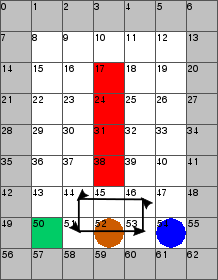
\includegraphics[scale = 0.5]{mdp_moveobs.png}
\caption{Gridworld with a moving obstacle}\label{fig:exp1}
\end{figure}
The state space of the agent is $(x,y,x_{obs},y_{obs})$ where the last two coordinates form the position of the moving obstacle. We assume that the state of the moving obstacle to be expensive to observe. Intuitively we expect to see if that we set the $\beta$ parameter high, \ie if the cost of information is high, the agent will go the long way around the wall as it will be too expensive to observe the moving obstacle. If the agent knows the position of the moving obstacle at all times, it can easily avoid collision as the obstacle motion is deterministic.
